\documentclass[conference]{IEEEtran}
\IEEEoverridecommandlockouts

\usepackage{cite}
\usepackage{amsmath,amssymb,amsfonts}
\usepackage{algorithm}
\usepackage{algorithmic}
\usepackage{graphicx}
\usepackage{textcomp}
\usepackage{booktabs}
\usepackage[caption=false,font=footnotesize]{subfig}
\usepackage{hyperref}
\hypersetup{
    colorlinks=true,
    citecolor=blue,
    linkcolor=red,
    urlcolor=blue
}
\usepackage{url}
\usepackage{xurl}
\usepackage{capt-of}
\usepackage[table]{xcolor}
\usepackage{colortbl}
\usepackage{tabularx}
\usepackage{soul}
\usepackage{multirow}
\usepackage{enumitem}
\usepackage{tikz}
\usepackage{pgfplots}
\pgfplotsset{compat=1.18}

\Urlmuskip=0mu plus 1mu

% Model colors
\definecolor{LlamaColor}{RGB}{78,121,167}
\definecolor{MistralColor}{RGB}{242,142,43}
\definecolor{Qwen25Color}{RGB}{89,161,79}
\definecolor{Qwen3Color}{RGB}{76,183,172}
\definecolor{GemmaColor}{RGB}{176,122,161}
\definecolor{PhiColor}{RGB}{225,87,89}

% Baseline colors
\definecolor{DeepCTIColor}{RGB}{76,120,168}
\definecolor{RAGColor}{RGB}{89,161,79}
\definecolor{EqualEvidenceColor}{RGB}{242,142,43}
\definecolor{NoMemoryColor}{RGB}{176,122,161}
\definecolor{OneShotColor}{RGB}{150,150,150}

% Table heatmap colors
\definecolor{TableHeader}{RGB}{230,239,248}
\definecolor{QualA}{RGB}{238,247,253}
\definecolor{QualB}{RGB}{218,236,249}
\definecolor{QualC}{RGB}{194,222,243}
\definecolor{QualBest}{RGB}{165,207,235}
\definecolor{StableGreen}{RGB}{224,243,230}
\definecolor{LatOne}{RGB}{229,244,233}
\definecolor{LatTwo}{RGB}{237,244,222}
\definecolor{LatThree}{RGB}{247,237,211}
\definecolor{LatFour}{RGB}{250,222,202}
\definecolor{TokOne}{RGB}{240,235,250}
\definecolor{TokTwo}{RGB}{229,219,245}
\definecolor{TokThree}{RGB}{216,201,238}
\definecolor{TokFour}{RGB}{203,184,229}

% Table cell formatting commands
\newcommand{\qA}[1]{\cellcolor{QualA}#1}
\newcommand{\qB}[1]{\cellcolor{QualB}#1}
\newcommand{\qC}[1]{\cellcolor{QualC}#1}
\newcommand{\qBest}[1]{\cellcolor{QualBest}\textbf{#1}} 
\newcommand{\stable}[1]{\cellcolor{StableGreen}#1}
\newcommand{\latone}[1]{\cellcolor{LatOne}\textbf{#1}}
\newcommand{\lattwo}[1]{\cellcolor{LatTwo}#1}
\newcommand{\latthree}[1]{\cellcolor{LatThree}#1}
\newcommand{\latfour}[1]{\cellcolor{LatFour}#1}
\newcommand{\tokone}[1]{\cellcolor{TokOne}\textbf{#1}}  
\newcommand{\toktwo}[1]{\cellcolor{TokTwo}#1}
\newcommand{\tokthree}[1]{\cellcolor{TokThree}#1}
\newcommand{\tokfour}[1]{\cellcolor{TokFour}#1}

% Author comments & highlights
\newcommand{\subash}[1]{{\color{blue}~{\em Comment by Subash: #1}}}
\DeclareRobustCommand{\hlcyan}[1]{{\sethlcolor{cyan!30}\hl{#1}}}
\DeclareRobustCommand{\hlred}[1]{{\sethlcolor{red!30}\hl{#1}}}

\begin{document}

\title{DeepCTI: Evidence State Control for Threat Mitigation Decisions}


% Double-blind submission: leave author block blank or anonymized
\author{
\IEEEauthorblockN{Anonymous Author(s)}
\IEEEauthorblockA{Anonymous Institution}
}

\maketitle
\begin{abstract}
Cyber Threat Intelligence (CTI) provides information about threats and possible mitigations, but a mitigation decision depends on the state of the local environment. Missing, conflicting, or outdated observations can leave vulnerability applicability and operational conditions unresolved. We argue that CTI-driven mitigation should be governed by an explicit evidence state that preserves supporting observations, identifies information gaps, and records how new evidence changes the assessment. Permission to investigate or modify the environment should additionally depend on organizational policy and current operational context. We present DeepCTI, a framework that implements evidence-state management by separating deterministic decision control from language-model synthesis. DeepCTI combines public CTI with local observations, maintains structured fact memory, and validates analyst-facing responses through bounded repair and deterministic fallback. A controlled study uses 100 synthetic vulnerability-centered cases across six locally deployed language models, producing 600 model--case runs. Applicability accuracy was 1.000, and mean composite quality ranged from 0.886 to 0.925. In a matched comparison across three models and five execution modes, DeepCTI achieved mean quality of 0.907, compared with 0.808 for RAG once, 0.805 for equal-evidence one-shot, 0.803 for iterative no-memory, and 0.605 for initial one-shot. These findings provide preliminary evidence for structured state management under staged observations. We develop a research agenda connecting this evidence process to current-state verification, conflict reconciliation, and contextual action authorization.
\end{abstract}

\begin{IEEEkeywords}
Cyber Threat Intelligence, Mitigation Decision Support, Evidence State Management, Large Language Models, Action Authorization
\end{IEEEkeywords}

\section{Introduction}

Cyber Threat Intelligence (CTI) provides information about
vulnerabilities, affected products, exploitation activity, and possible
mitigations. Public sources such as vulnerability databases and vendor
advisories help explain a threat, but mitigation decisions depend on
local facts such as product presence, installed version, rollback
capability, and deployment constraints. Prior work on security patch
management shows that remediation also depends on testing, coordination,
and service availability~\cite{dissanayake2022automation,jenkins2024patching,souppaya2022patchmanagement}.

Consider an advisory affecting a product listed in an organization's
inventory, where the product's active version has not been verified. A decision-support
system should identify the version check as an information need and
update its applicability assessment when the observation becomes
available. A later configuration change or conflicting observation may
require reassessment. Even when evidence supports mitigation, permission
to perform a disruptive change depends on organizational policy and
current operating conditions. Configuration monitoring and
attribute-based access control provide foundations for these
requirements~\cite{johnson2011configuration,dempsey2011monitoring,hu2014abac}.
The system must therefore determine both \emph{what information is
still needed} and \emph{how new evidence changes the assessment}.

Retrieval-augmented generation improves access to external
information~\cite{lewis2020rag}, while ReAct and Toolformer support
information gathering through external
tools~\cite{yao2023react,schick2023toolformer}. LocalIntel combines
general cyber knowledge with organization-specific information to
generate contextualized threat intelligence~\cite{mitra2024localintel}.
For mitigation decision support, this information must be connected
to the facts required to assess the target environment. We argue that
CTI-driven mitigation should be governed by an explicit evidence state
that preserves observations, distinguishes established facts from
missing or conflicting information, and records changes to the
assessment. Recommendation eligibility and action authorization should
be evaluated separately: evidence supports the mitigation judgment,
while policy determines permitted actions. Recent agent security
research similarly treats tool permissions and runtime enforcement
as explicit controls~\cite{shi2025progent,wang2026agentspec}.

This position leads to two research questions.

\textbf{RQ-1:}
Which facts and relationships in an evolving evidence state establish
local applicability, identify unresolved information, and support a
mitigation recommendation as new observations become available?

\textbf{RQ-2:}
How should evidence-based mitigation judgments be connected to current
operational context and policy so that investigative and mitigation
actions remain within the agent's authorization?

We present \textbf{DeepCTI}, a framework that combines public CTI with
source-linked local observations in a structured evidence state.
A deterministic controller tracks known, unknown, and conflicting
facts to produce applicability assessments and information needs.
Language-model synthesis produces an analyst-facing response checked
through validation, bounded repair, and deterministic fallback.
The controlled study examines evidence-state behavior within RQ-1
using staged observations across local language models and alternative
execution modes. The requirements of RQ-2 are developed through an
operational research agenda.

This paper makes three contributions:
\begin{itemize}
    \item We formulate mitigation as an evolving evidence-dependent
    decision process, connecting local applicability, information gaps,
    and new observations to recommendation conditions, while
    distinguishing these conditions from authorization to act.

    \item We present DeepCTI, combining source-linked observations,
    structured fact memory, deterministic decision rules, and validated
    synthesis. We evaluate its behavior across six local language models
    and compare it with four alternative execution modes, assessing
    applicability, response quality, unresolved information, and
    computational cost.

    \item We develop a research agenda for current-state verification,
    evidence reconciliation, and contextual action authorization,
    connecting these requirements to evaluation criteria for evidence
    support, decision progress, and authorization compliance.
\end{itemize}

The remainder of the paper is organized as follows. Section~II reviews
related work. Section~III presents DeepCTI, Section~IV describes the
experimental methodology, and Section~V reports the results.
Section~VI discusses the findings, research agenda, and limitations.
Section~VII concludes the paper.

\section{Related Work}

\subsection{Cyber Threat Intelligence and Mitigation}

CTI systems help analysts interpret vulnerabilities, attacks, and
possible responses. LocalIntel combines global cyber knowledge with
organization-specific information to generate contextualized threat
intelligence~\cite{mitra2024localintel}. DeepCTI shares this use of local
context and examines how observations support applicability assessments
and further verification. TrustOps also proposes evidence-grounded
cyber defence with consideration of missing, conflicting, stale, and
low-confidence evidence~\cite{malamas2026trustops}. These approaches
motivate examining how evidence is represented and connected to a
mitigation decision.

Mitigation involves operational conditions that may not appear in an
advisory. Patch-management studies report challenges involving testing,
coordination, deployment delays, and service
availability~\cite{dissanayake2022automation,dissanayake2022delays,jenkins2024patching}.
Li and Paxson examine practical reliability concerns associated with
security patches~\cite{li2017securitypatches}, while NIST guidance
addresses planning, prioritization, testing, and
deployment~\cite{souppaya2022patchmanagement}. These findings support
including local operational conditions in mitigation analysis.

Local information must also remain relevant as the environment changes.
NIST configuration management and continuous monitoring guidance
addresses maintaining system information and observing configuration
changes~\cite{johnson2011configuration,dempsey2011monitoring}.
An inventory or version observation may therefore require verification
before it supports a current mitigation decision.

Several benchmarks examine complementary CTI capabilities. CTIBench
evaluates cybersecurity knowledge and reasoning~\cite{alam2024ctibench}.
AthenaBench includes a Risk Mitigation Strategy task mapping attack
descriptions to mitigation identifiers~\cite{alam2025athenabench}.
CTIConnect evaluates retrieval-augmented reasoning over heterogeneous
CTI sources~\cite{cheng2025cticonnect}, while ExCyTIn-Bench evaluates
interactive threat investigation~\cite{wu2025excytin}. Local mitigation
evaluation additionally requires explicit asset applicability,
operational constraints, evidence conditions, and permissions to act.

\subsection{Retrieval Approaches for Augmented Generation}

Retrieval-augmented generation (RAG) grounds model outputs in external
information~\cite{lewis2020rag}. BM25 ranks documents through lexical
correspondence~\cite{robertson2009bm25}, while dense retrieval uses
learned query and passage representations~\cite{karpukhin2020dense}.
GraphRAG supports query-focused summarization over graph-structured
collections, and HybridRAG combines graph and vector
retrieval~\cite{edge2024graphrag,sarmah2024hybridrag}.

Retrieved information also requires assessment. Self-RAG retrieves and
reflects on evidence as needed, while Corrective RAG assesses retrieval
quality before generation~\cite{asai2024selfrag,yan2024crag}.
Misleading retrieved content can adversely affect model
responses~\cite{hong2024gullible}. For mitigation analysis, even an
accurate advisory does not establish local product presence or version
status. LocalIntel addresses contextualization through public and
organization-specific information~\cite{mitra2024localintel}.
An explicit evidence state connects these observations to decision
requirements and identifies remaining information gaps.

Reasoning approaches organize analysis across multiple steps. Direct
prompting supplies the task in a single prompt, while Chain-of-Thought
introduces intermediate reasoning~\cite{wei2022cot}. Tree of Thoughts
explores alternative paths, and Reasoning via Planning applies planning
and search~\cite{yao2023tot,hao2023rap}. Chain-of-Reasoning combines
reasoning paradigms for mathematical tasks~\cite{yu2025cor}.
ReAct interleaves reasoning with external actions, while Toolformer
learns when and how to invoke tools~\cite{yao2023react,schick2023toolformer}.
The Paper Assistant Tool illustrates decomposition, search grounding,
and coordinated analysis in scientific review~\cite{jayaram2026pat}.

Retrieval can also adapt as reasoning progresses. IRCoT interleaves
retrieval with intermediate reasoning, while Adaptive-RAG selects
retrieval strategies according to question
complexity~\cite{trivedi2023ircot,jeong2024adaptiverag}.
DeepCTI connects information needs to an explicit fact state and
incorporates incoming observations. Its controlled study uses
predefined evidence stages to examine state management separately
from autonomous acquisition.

\subsection{Memory, Evidence Freshness, and Verification}

MemGPT studies memory management for long-running language-model
applications~\cite{packer2023memgpt}. In mitigation analysis, retained
observations must also remain connected to their asset, source, and
the decision they support.

FreshLLMs examines access to current information as knowledge
changes~\cite{vu2024freshllms}. Temporal conflict analysis and EvoTrustRAG
examine conflicting or evolving evidence in retrieval-based
systems~\cite{ozer2025temporalconflict,nie2026evotrustrag}.
These studies motivate considering evidence validity alongside
retention: a new observation may refine an assessment, indicate a
system change, or introduce a disagreement requiring investigation.

Verification provides additional response checks. Self-RAG supports
reflection on retrieved information, while Chain-of-Verification with
retrieval examines checking and revision of generated
outputs~\cite{asai2024selfrag,he2024covrag}. DeepCTI places response
verification after evidence-state management. The controller establishes
applicability, and the verifier checks agreement with that assessment
and references to available evidence. Its memory preserves conflicts;
current-state verification and temporal validity form part of the
operational agenda in Section~VI.

\subsection{Contextual Authorization and Agent Action Control}

A supported mitigation judgment and permission to execute an action
are distinct requirements. Attribute-based access control evaluates
subject, object, action, and environmental attributes against
policy~\cite{hu2014abac}. NIST guidance addresses the reliability and
management of these attributes~\cite{hu2019attributes}. Least privilege
and complete mediation provide foundations for restricting authority
and checking access~\cite{saltzer1975protection}.

Recent agent systems develop explicit tool controls. Progent applies
privilege control to tool names and arguments, while AgentSpec uses
runtime rules to constrain actions~\cite{shi2025progent,wang2026agentspec}.
CaMeL separates trusted control from untrusted data flows, and DRIFT
examines dynamic constraints and isolation~\cite{debenedetti2025camel,li2025drift}.
A framework for formalizing agent security distinguishes action
alignment, source authorization, and data isolation~\cite{siu2026agentsecurity}.
These approaches inform the connection between an assessment and
an enforceable action policy.

For CTI-driven mitigation, observations supply policy inputs such as
asset identity, configuration, and approval status. Organizational
policy determines permission to investigate or modify the environment.
Retrieved content therefore provides evidence rather than authority.
DeepCTI's operational agenda connects its evidence state to this
authorization requirement.

AgentDojo and InjecAgent evaluate indirect prompt injection in
tool-using settings~\cite{debenedetti2024agentdojo,zhan2024injecagent}.
ToolEmu examines risks in an emulated sandbox, while R-Judge evaluates
risk recognition~\cite{ruan2024toolemu,yuan2024rjudge}.
Research on injection benchmarks identifies weaknesses in attack
construction and scoring~\cite{bhagwatkar2025injectionbenchmarks}.
These studies motivate measuring both useful progress and compliance
with action constraints.

Together, this literature grounds contextual CTI, information
acquisition, evidence management, and action control. Section~III
presents DeepCTI's evidence-state pipeline, while Section~VI develops
its operational extensions.

\section{DeepCTI}

DeepCTI supports vulnerability mitigation decisions using public CTI
and local observations. As shown in Figure~\ref{fig:architecture},
source-linked observations enter structured memory, and a deterministic
controller evaluates applicability, information needs, and stopping
conditions. Cases with resolved applicability proceed to language-model synthesis and validation unresolved cases return a deterministic verification
request. The model communicates the assessment without changing the
controller's applicability state. This pipeline implements evidence-state
management, while current-state verification and contextual authorization
are developed in Section~VI.

\begin{table}[!t]
\caption{Main notation used in DeepCTI.}
\label{tab:notation}
\centering
\scriptsize
\setlength{\tabcolsep}{3.5pt}
\renewcommand{\arraystretch}{1.08}
\begin{tabularx}{\columnwidth}{
    >{\centering\arraybackslash}p{0.18\columnwidth}
    >{\raggedright\arraybackslash}X
}
\toprule
\textbf{Symbol} & \textbf{Meaning} \\
\midrule
$R$ & Public CTI information. \\
$L$ & Local context for the target environment. \\
$E$ & Set of collected observations. \\
$S$ & Current evidence state. \\
$S_f$ & State of fact slot $f$. \\
$A(S)$ & Applicability assessment from state $S$. \\
$P$ & Product-presence state. \\
$V$ & Version-status state. \\
$n_{\mathrm{abs}}$ & Number of distinct evidence identifiers supporting product absence. \\
$R_b$ & Rollback status. \\
$s(c,e)$ & Lexical support score between claim $c$ and evidence $e$. \\
$\mathrm{Acc}_{\mathrm{app}}$ & Applicability accuracy. \\
$R_{\mathrm{unsafe}}$ & Case-defined forbidden-action lexical rate. \\
$R_{\mathrm{comp}}$ & Completion rate. \\
$q_i$ & Composite quality score for case $i$. \\
$Q$ & Mean composite quality across evaluated cases. \\
\bottomrule
\end{tabularx}
\end{table}

\subsection{Problem Formulation}

For a vulnerability-centered case, let $R$ denote public CTI,
$L$ the available local context, and $E=\{e_1,\ldots,e_n\}$ the
collected observations. DeepCTI maintains an evidence state $S$
and produces an analyst-facing response describing applicability,
conditional mitigation, or further verification. The implementation
records product presence, version status, rollback availability, and
change approval through deterministic extraction rules.

The assessment distinguishes four conditions. An applicable state
establishes that the product is installed and its version is affected.
A non-applicable state establishes product absence. A potentially
applicable state indicates product presence without an established
affected version. Conflicting product or version observations, or
unresolved product presence, lead to an uncertain state. DeepCTI
provides decision support and does not execute changes to the environment.

\subsection{Observation and State Representation}

Each observation records a fact field, normalized value, evidence
identifier, source type, reliability level, and evaluation step.
Observations are grouped into fact slots, preserving earlier records
as new evidence arrives. For a slot $f$,

\begin{equation}
S_f =
\begin{cases}
\text{conflict}, & \text{if exclusive values exist},\\
\text{unknown}, & \text{if no known value exists},\\
v^{*}, & \text{otherwise}.
\end{cases}
\label{eq:slot}
\end{equation}

Here, $v^{*}$ is the resolved value. Compatible observations are ranked
by source reliability, with the latest evidence step breaking ties.
The order is primary, authoritative, secondary, and unknown.
The evaluation step represents processing order rather than verified
real-world freshness.

Learning that an unknown version is affected refines the state,
whereas observations indicating both product presence and absence create
a conflict.
The mutually exclusive pairs are
\texttt{installed}/\texttt{not\_installed},
\texttt{affected}/\texttt{unaffected},
\texttt{available}/\texttt{unavailable}, and
\texttt{approved}/\texttt{withheld}. Conflicting observations are
retained and the slot is marked accordingly. Content hashes identify
duplicate records so repeated content is not counted as new evidence.

\subsection{Decision Controller}

After each update, the controller evaluates applicability using
product presence $P$ and version status $V$. For states without
product or version conflicts,

\begin{equation}
A(S)=
\begin{cases}
\text{applicable}, &
P=\text{installed},\; V=\text{affected},\\
\text{not applicable}, &
P=\text{not installed},\\
\text{potential}, &
P=\text{installed},\; V\neq\text{affected},\\
\text{uncertain}, &
\text{otherwise}.
\end{cases}
\label{eq:applicability}
\end{equation}

Here, \textit{potential} denotes the potentially applicable state.
Product or version conflicts take precedence and produce an uncertain
state. The current rules establish non-applicability through product
absence; an installed but unaffected version has no separate
non-applicability branch.

The controller separately evaluates stopping conditions. For a
non-applicable case, $n_{\mathrm{abs}}$ counts distinct evidence
identifiers supporting product absence:

\begin{equation}
C_{\mathrm{NA}}
=
\bigl(A(S)=\text{not applicable}\bigr)
\land
\bigl(n_{\mathrm{abs}}\geq 2\bigr).
\label{eq:na_sufficient}
\end{equation}

Distinct identifiers do not establish independence between sources.
For an applicable case, rollback status $R_b$ must be known:

\begin{equation}
C_{\mathrm{A}}
=
\bigl(A(S)=\text{applicable}\bigr)
\land
\bigl(R_b\in\{\text{available},\text{unavailable}\}\bigr).
\label{eq:a_sufficient}
\end{equation}

Either condition permits processing to stop. An unavailable rollback
plan resolves the fact slot but remains an operational constraint.

Information needs accompany these assessments. Unresolved product
presence prompts an installation check; unresolved version status
prompts verification against affected versions. Conflicting observations
produce reconciliation requests. When product absence is not established
and rollback is unavailable or unresolved, the controller requests
rollback capability before a state-changing mitigation.

Processing also ends when the step budget is exhausted or no novel
evidence is available. The final branch uses applicability to select
synthesis or a deterministic verification request, without separately
enforcing every stopping condition. Resolved cases in the controlled
profiles reach the specified stopping conditions.

Change approval is retained as response context but is not enforced
as a stopping or execution condition. Evidence resolution supports
the assessment; permission to execute requires a policy decision.

\subsection{Generation, Verification, and Deterministic Fallback}

For cases with resolved applicability, the local language model receives the
evidence state and observations and produces a structured response. Validation checks agreement with the controller's applicability
assessment, the presence of a final answer, references to available
evidence, the occurrence of case-defined forbidden-action phrases,
and textual support for claims

For claim $c$ and cited record $e$, lexical support is

\begin{equation}
s(c,e)=
\frac{|T(c)\cap T(e)|}{|T(c)|},
\label{eq:overlap}
\end{equation}

where $T(\cdot)$ denotes the token set extracted by the verifier. For multiple citations,

\begin{equation}
s(c)=\max_{e\in E_c}s(c,e),
\label{eq:claimscore}
\end{equation}

where $E_c$ contains the records cited by $c$.

A claim is classified as supported when $s(c)\geq 0.55$, partially
supported when $0.25\leq s(c)<0.55$, and unsupported below $0.25$.
Missing or invalid identifiers also produce an unsupported
classification. Scoped negation conflicts with sufficient lexical
overlap are classified as contradicted. These checks identify missing
references, weak textual support, and polarity conflicts; they provide
lexical verification rather than semantic entailment or authorization.

A response that fails validation receives one repair attempt using the
reported errors. If the revised response fails the same checks, a deterministic
fallback replaces it. Unresolved applicability follows the verification
path directly without a model call. Recorded states, observations,
contradictions, information needs, generation attempts, validation
outcomes, token usage, and fallbacks distinguish controller behavior
from synthesis and verification outcomes.

\subsection{Illustrative End-to-End Use Case}
\label{sec:illustrative-use-case}

Figure~\ref{fig:printnightmare_usecase} illustrates a PrintNightmare
mitigation scenario separately from the quantitative evaluation.
Public intelligence supplies the threat description, while inventory
and version observations establish local applicability. Missing or
conflicting facts generate verification needs, and subsequent
observations update the assessment while preserving source relationships.

The scenario also considers patch and reboot requirements, printing
dependencies, Group Policy settings, change windows, and rollback.
These details illustrate the context needed to compare mitigation
options. The implemented controller represents product presence,
version status, rollback, and approval; the additional details
describe the broader operational use case.

Cases with resolved applicability follow the synthesis and validation
path, with bounded repair and fallback when needed. Operational execution additionally requires
current-state verification and a policy decision, as developed
in Section~VI.

\begin{figure*}[t]
    \centering
    \includegraphics[
        width=0.97\textwidth,
        keepaspectratio
    ]{figs/DeepCTI_Usecase.pdf}
    \caption{Illustrative PrintNightmare mitigation workflow.
    Public CTI and local observations inform an evolving assessment.
    The broader configuration and action analysis illustrates
    operational context beyond the implemented fact slots.}
    \label{fig:printnightmare_usecase}
\end{figure*}

\section{Experimental Methodology}

We conduct a controlled study of DeepCTI using vulnerability-centered
cases that represent different local information conditions. The study
examines applicability assessment, identification of unresolved
information, response quality, validation behavior, and computational
cost. It evaluates evidence-state behavior within RQ-1 and provides
preliminary findings for the operational research agenda.

\subsection{Dataset and Context Profiles}

The evaluation uses 100 cases generated deterministically from a local
snapshot of the CISA Known Exploited Vulnerabilities (KEV)
catalog~\cite{cisa_kev}. The first 100 records ordered by CVE identifier
provide the base vulnerability cases. KEV supplies public vulnerability
information, while synthetic local profiles supply the asset conditions
needed to examine mitigation decisions.

Each case represents one of four profiles: affected, not applicable,
uncertain, or contradictory. The dataset contains 25 cases per profile,
giving equal representation to cases with resolved and unresolved
applicability.

In an affected case, the product is installed and its version is
affected. A not-applicable case establishes product absence through
the required negative observations. An uncertain case contains
unresolved information needed to assess applicability. A contradictory
case contains mutually exclusive observations for a decision-relevant
fact. These profiles allow the controller's behavior to be examined
under defined evidence conditions.

Each case includes initial evidence and additional observations
introduced through predefined stages. Every model receives the same
cases and evidence sequence, with a maximum of three evidence-processing
steps per case. This design provides a reproducible comparison of
state updates and response behavior.

Expected applicability labels and keyword references are generated
with the profiles. They provide controlled reference conditions rather
than independently annotated operational judgments. Reference answers
are withheld from generation prompts. Case-defined forbidden phrases
are also used by the response validator, and validation errors can be
supplied during repair. Table~\ref{tab:deepcti-dataset-schema} summarizes
the case structure.

\begin{table}[!t]
\caption{Structure of a DeepCTI-KEV evaluation case.}
\label{tab:deepcti-dataset-schema}
\centering
\scriptsize
\setlength{\tabcolsep}{3.2pt}
\renewcommand{\arraystretch}{1.08}
\begin{tabularx}{\columnwidth}{
    >{\raggedright\arraybackslash}p{0.30\columnwidth}
    >{\raggedright\arraybackslash}X
}
\toprule
\textbf{Field} & \textbf{Description} \\
\midrule
\texttt{case\_id}
& Unique identifier for the evaluation case. \\
\texttt{cve\_id}
& KEV vulnerability associated with the case. \\
\texttt{profile\_kind}
& Local profile: affected, not applicable, uncertain, or contradictory. \\
\texttt{question}
& Analyst-facing applicability and mitigation question. \\
\texttt{initial\_evidence}
& Public CTI and initial local observations available at step~0. \\
\texttt{staged\_evidence}
& Additional local observations introduced during later steps. \\
\texttt{reference}
& Expected applicability, action terms, information needs, forbidden phrases, and contradiction status. \\
\bottomrule
\end{tabularx}
\end{table}

\subsection{Models and Experimental Configuration}

The cross-model experiment evaluates six locally deployed language
models: Llama 3.1 8B, Qwen 2.5 7B, Mistral, Qwen 3 8B, Gemma 3 12B,
and Phi-4 14B. All models run through Ollama with the same DeepCTI
controller configuration. Each model processes all 100 cases, producing
600 model--case records.

Generation uses a temperature of 0.00 and a maximum output length of
1,024 tokens. The maximum evidence-processing budget is three steps,
the experiment seed is 20260819, and retrieval depth is $k=8$ where
retrieval is used. Experiment manifests retain model identifiers,
digests, configuration values, and dataset hashes.

The cross-model comparison examines whether applicability and response
behavior remain consistent when the synthesis model changes. Completed
runs are stored as JSONL records. The runner supports resuming
incomplete experiments while retaining previously completed records.

\subsection{Controlled Mode Comparison}

A separate matched comparison evaluates DeepCTI and four alternative
execution modes using the same 100 cases. It includes Llama 3.1 8B,
Qwen 2.5 7B, and Mistral. Each model processes every case under five
modes, producing 1,500 executions.

The modes are:
\begin{itemize}
    \item \textbf{DeepCTI:} structured fact memory, conflict handling,
    deterministic applicability assessment, response validation,
    bounded repair, and deterministic fallback.

    \item \textbf{Equal-evidence one-shot:} all available case evidence
    is supplied in one prompt, controlling for total information
    availability.

    \item \textbf{RAG once:} one retrieval step selects information
    from the complete case evidence pool before generation.

    \item \textbf{Iterative no-memory:} evidence is introduced across
    repeated steps without retaining the generated state between
    steps.

    \item \textbf{Initial one-shot:} generation uses only the initial
    CTI and local observations, without later evidence.
\end{itemize}

All modes use the same cases, model settings, and applicable processing
budgets. Each model--mode combination contains 100 cases, enabling
matched comparisons. The comparison evaluates the complete execution
strategies; differences can therefore reflect their combined
state-management, prompting, and response-control behavior.

\subsection{Evaluation Metrics}

The evaluation measures applicability correctness, information-need
identification, action terms, forbidden-action lexical matches,
contradiction handling, completion, and computational cost.

\textit{Applicability accuracy} measures the proportion of cases whose
final applicability state matches the reference label. For $N$ cases,

\begin{equation}
\mathrm{Acc}_{\mathrm{app}}
=
\frac{1}{N}
\sum_{i=1}^{N}
\mathbb{I}\left(\hat{A}_i=A_i^{*}\right),
\label{eq:app_accuracy}
\end{equation}

where $\hat{A}_i$ is the final assessment, $A_i^{*}$ is the expected
label, and $\mathbb{I}(\cdot)$ is the indicator function.

For lexical scoring, let $T_i$ denote the combined final answer,
selected action, and reported information needs for case $i$.
\textit{Action-keyword recall} measures the presence of action terms
specified in the reference:

\begin{equation}
R_i^{A}
=
\frac{1}{|K_i^{A}|}
\sum_{k\in K_i^{A}}
\mathbb{I}\left(k\text{ occurs in }T_i\right),
\label{eq:action_recall}
\end{equation}

where $K_i^{A}$ is the set of expected action keywords.

\textit{Information-need keyword recall} measures the presence of
terms identifying the expected missing or conflicting information:

\begin{equation}
R_i^{I}
=
\frac{1}{|K_i^{I}|}
\sum_{k\in K_i^{I}}
\mathbb{I}\left(k\text{ occurs in }T_i\right),
\label{eq:information_recall}
\end{equation}

where $K_i^{I}$ is the reference set of information-need keywords.
Both recall measures use case-insensitive substring matching.
For composite scoring, a recall component is assigned 1.0 when its
reference keyword set is empty. Information-need recall is interpreted
as an identification measure for cases with non-empty references.

\textit{Forbidden-action lexical rate}, retained as
\textit{unsafe-action rate} in the existing result records, measures
whether $T_i$ contains a forbidden phrase specified by the reference:

\begin{equation}
R_{\mathrm{unsafe}}
=
\frac{1}{N}
\sum_{i=1}^{N}
\mathbb{I}(u_i=1),
\label{eq:unsafe_rate}
\end{equation}

where $u_i=1$ indicates at least one forbidden-phrase match.
This measure concerns the specified output terms. Execution
authorization and operational safety require separate evaluation.

\textit{Contradiction correctness} measures whether the detected
contradiction status matches the reference. The scorer marks a
contradiction as detected when the final state contains contradiction
records or $T_i$ contains one of the cues \texttt{contradict},
\texttt{conflict}, or \texttt{reconcile}. This lexical component is
considered alongside the recorded evidence state.

\textit{Completion rate} measures the proportion of records marked as
completed:

\begin{equation}
R_{\mathrm{comp}}
=
\frac{1}{N}
\sum_{i=1}^{N}
\mathbb{I}(c_i=1),
\label{eq:completion_rate}
\end{equation}

where $c_i=1$ indicates completion according to the execution mode's
recorded criteria. A deterministic DeepCTI response counts as completed
when it satisfies its final validation requirements. Completion
therefore includes verification requests and fallback responses.

The \textit{composite quality score} summarizes five components:
applicability correctness, action-keyword recall, information-need
keyword recall, absence of forbidden-action matches, and contradiction
correctness. For case $i$,

\begin{equation}
q_i
=
\frac{1}{5}
\sum_{j=1}^{5}q_{i,j},
\label{eq:case_quality}
\end{equation}

where $q_{i,j}$ denotes the value of component $j$ for case $i$. Mean quality is

\begin{equation}
Q
=
\frac{1}{N}
\sum_{i=1}^{N}q_i.
\label{eq:mean_quality}
\end{equation}

This score is a project-specific summary of behavior on the controlled
profiles. Individual measures are reported alongside it to distinguish
applicability, information needs, and lexical response behavior.

Computational cost is measured through median recorded model latency
and median token usage across cases. Latency is the sum of durations
reported by Ollama for the model calls within a case, including repair
when attempted. Token usage includes prompt and completion tokens
across those calls. Cases without a model call record zero model
duration and tokens. These measures characterize inference cost rather
than the full time required for operational investigation.

\subsection{Validation, Repair, and Fallback Analysis}

The evaluation records response-validation behavior separately from
final quality. For each model, the 50 cases with resolved applicability
are divided into three outcomes: acceptance on initial generation,
recovery through one repair attempt, or replacement with a deterministic
fallback.

The 50 unresolved cases follow the deterministic verification path
without a language-model call. These cases are analyzed separately
from generation failures because the response follows directly from
the unresolved applicability state. The recorded outcomes distinguish
controller decisions, synthesis behavior, and the effect of response
validation.

\subsection{Statistical Analysis}

For the six-model experiment, uncertainty in mean composite quality is
estimated using 20,000 bootstrap resamples over the 100 cases.
Each resample selects cases with replacement and recomputes the mean.
The 2.5th and 97.5th percentiles define the 95\% confidence interval.
Applicability accuracy, forbidden-action lexical rate, and completion
rate are reported directly over the fixed evaluation set.

For the matched mode comparison, the case is the statistical unit.
Quality is first averaged across the three models for each case and
mode. Bootstrap resampling then operates over the 100 cases,
preserving their grouping across models. The resulting percentile
intervals describe uncertainty in the case-level mean quality.

Pairwise comparisons use the 100 matched case-level quality
differences between DeepCTI and each alternative mode. Two-sided
sign-flip tests use 100,000 random sign assignments. The four resulting
$p$-values are corrected jointly using the Holm procedure, with
statistical significance evaluated at $\alpha=0.05$.

\section{Results}

\subsection{Overall Performance Across Models}

DeepCTI completed all 100 cases for each of the six evaluated models,
producing 600 completed model--case runs. Applicability accuracy was
1.000 for every model, the forbidden-action lexical rate was 0.00,
and the completion rate was 1.000. Table~\ref{tab:main_results} reports
the measures that varied with model choice.

\begin{table}[!ht]
\caption{Model-level performance across the 100-case DeepCTI evaluation.
Tokens are medians across cases.}
\label{tab:main_results}
\centering
\scriptsize
\setlength{\tabcolsep}{4pt}
\renewcommand{\arraystretch}{1.12}
\begin{tabularx}{\columnwidth}{
    >{\hsize=1.0\hsize\raggedright\arraybackslash}X
    >{\hsize=1.2\hsize\centering\arraybackslash}X
    >{\hsize=0.8\hsize\centering\arraybackslash}X
}
\toprule
\textbf{Model} &
\textbf{Quality [95\% CI]} &
\textbf{Tokens} \\
\midrule
\rowcolor{LlamaColor!14}
Llama 3.1 8B &
0.886 [0.862, 0.909] &
\textbf{509.5} \\
\rowcolor{MistralColor!14}
Mistral &
0.910 [0.884, 0.934] &
704.0 \\
\rowcolor{Qwen25Color!14}
Qwen 2.5 7B &
\textbf{0.925 [0.898, 0.949]} &
602.0 \\
\rowcolor{Qwen3Color!14}
Qwen 3 8B &
0.923 [0.897, 0.948] &
598.0 \\
\rowcolor{GemmaColor!14}
Gemma 3 12B &
\textbf{0.925 [0.898, 0.949]} &
626.5 \\
\rowcolor{PhiColor!14}
Phi-4 14B &
\textbf{0.925 [0.898, 0.949]} &
609.0 \\
\bottomrule
\end{tabularx}
\end{table}

Mean composite quality ranged from 0.886 to 0.925. Qwen 2.5 7B,
Gemma 3 12B, and Phi-4 14B reached the highest observed mean of
0.925, followed by Qwen 3 8B at 0.923. Mistral reached 0.910,
and Llama 3.1 8B reached 0.886. These values describe variation
in the complete DeepCTI responses across synthesis models. The
experiment does not establish a statistical ranking of the models.

Figure~\ref{fig:quality_latency} shows mean quality, its bootstrap
confidence interval, and recorded median model latency. The
applicability results remained unchanged across the six models,
consistent with the use of a shared deterministic controller.

\begin{figure}[!ht]
\centering
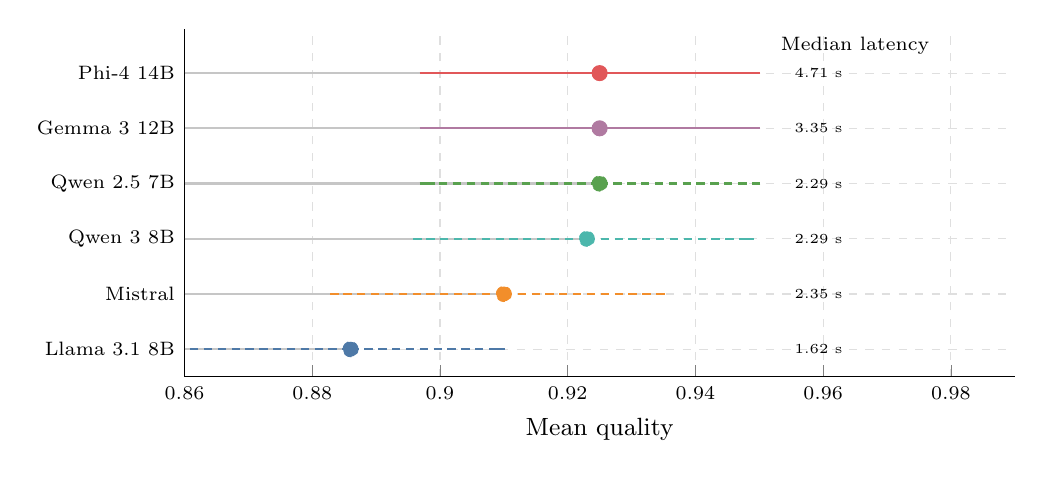
\begin{tikzpicture}
\begin{axis}[
    width=\columnwidth,
    height=6.0cm,
    xmin=0.86,
    xmax=0.99,
    ymin=0.5,
    ymax=6.8,
    xlabel={Mean quality},
    ytick={1,2,3,4,5,6},
    yticklabels={
        Llama 3.1 8B,
        Mistral,
        Qwen 3 8B,
        Qwen 2.5 7B,
        Gemma 3 12B,
        Phi-4 14B
    },
    tick label style={font=\scriptsize},
    label style={font=\small},
    yticklabel style={font=\scriptsize,align=right},
    grid=major,
    grid style={dashed,gray!25},
    axis x line*=bottom,
    axis y line*=left,
    clip=false
]
\addplot[gray!45,line width=0.8pt]
    coordinates {(0.86,1) (0.886,1)};
\addplot[gray!45,line width=0.8pt]
    coordinates {(0.86,2) (0.910,2)};
\addplot[gray!45,line width=0.8pt]
    coordinates {(0.86,3) (0.923,3)};
\addplot[gray!45,line width=0.8pt]
    coordinates {(0.86,4) (0.925,4)};
\addplot[gray!45,line width=0.8pt]
    coordinates {(0.86,5) (0.925,5)};
\addplot[gray!45,line width=0.8pt]
    coordinates {(0.86,6) (0.925,6)};

\addplot+[
    only marks,mark=*,mark size=2.7pt,
    mark options={fill=LlamaColor,draw=LlamaColor},
    error bars/.cd,x dir=both,x explicit,
    error bar style={draw=LlamaColor,line width=0.8pt},
    error mark options={draw=LlamaColor,line width=0.8pt}
] coordinates {(0.886,1) += (0.023,0) -= (0.024,0)};

\addplot+[
    only marks,mark=*,mark size=2.7pt,
    mark options={fill=MistralColor,draw=MistralColor},
    error bars/.cd,x dir=both,x explicit,
    error bar style={draw=MistralColor,line width=0.8pt},
    error mark options={draw=MistralColor,line width=0.8pt}
] coordinates {(0.910,2) += (0.024,0) -= (0.026,0)};

\addplot+[
    only marks,mark=*,mark size=2.7pt,
    mark options={fill=Qwen3Color,draw=Qwen3Color},
    error bars/.cd,x dir=both,x explicit,
    error bar style={draw=Qwen3Color,line width=0.8pt},
    error mark options={draw=Qwen3Color,line width=0.8pt}
] coordinates {(0.923,3) += (0.025,0) -= (0.026,0)};

\addplot+[
    only marks,mark=*,mark size=2.7pt,
    mark options={fill=Qwen25Color,draw=Qwen25Color},
    error bars/.cd,x dir=both,x explicit,
    error bar style={draw=Qwen25Color,line width=0.8pt},
    error mark options={draw=Qwen25Color,line width=0.8pt}
] coordinates {(0.925,4) += (0.024,0) -= (0.027,0)};

\addplot+[
    only marks,mark=*,mark size=2.7pt,
    mark options={fill=GemmaColor,draw=GemmaColor},
    error bars/.cd,x dir=both,x explicit,
    error bar style={draw=GemmaColor,line width=0.8pt},
    error mark options={draw=GemmaColor,line width=0.8pt}
] coordinates {(0.925,5) += (0.024,0) -= (0.027,0)};

\addplot+[
    only marks,mark=*,mark size=2.7pt,
    mark options={fill=PhiColor,draw=PhiColor},
    error bars/.cd,x dir=both,x explicit,
    error bar style={draw=PhiColor,line width=0.8pt},
    error mark options={draw=PhiColor,line width=0.8pt}
] coordinates {(0.925,6) += (0.024,0) -= (0.027,0)};

\node[font=\tiny,anchor=west] at (axis cs:0.954,1) {1.62 s};
\node[font=\tiny,anchor=west] at (axis cs:0.954,2) {2.35 s};
\node[font=\tiny,anchor=west] at (axis cs:0.954,3) {2.29 s};
\node[font=\tiny,anchor=west] at (axis cs:0.954,4) {2.29 s};
\node[font=\tiny,anchor=west] at (axis cs:0.954,5) {3.35 s};
\node[font=\tiny,anchor=west] at (axis cs:0.954,6) {4.71 s};
\node[font=\scriptsize,anchor=center]
    at (axis cs:0.965,6.5) {Median latency};
\end{axis}
\end{tikzpicture}
\caption{Mean composite quality and median model latency across
the six-model evaluation. Error bars show 95\% bootstrap
confidence intervals.}
\label{fig:quality_latency}
\end{figure}

\subsection{Validation, Repair, and Fallback Behavior}

Each model has 50 cases with resolved applicability that proceed to
language-model synthesis. Figure~\ref{fig:validation_paths} shows their
distribution across initial acceptance, successful repair, and
deterministic fallback.

Llama 3.1 8B and Qwen 3 8B each produced 46 responses accepted after the
initial generation. Mistral and Phi-4 14B each produced 36, while
Qwen 2.5 7B and Gemma 3 12B produced 40 and 43, respectively.
Repair recovered four cases for Qwen 2.5 7B and one case each for
Qwen 3 8B and Phi-4 14B. The remaining responses were replaced
with deterministic fallbacks.

Across the six models, all 300 uncertain or contradictory executions
followed the deterministic verification path without a model call.
These outcomes distinguish responses derived directly from unresolved
applicability from fallbacks following unsuccessful generation.

\begin{figure}[!t]
\centering
\resizebox{\columnwidth}{!}{
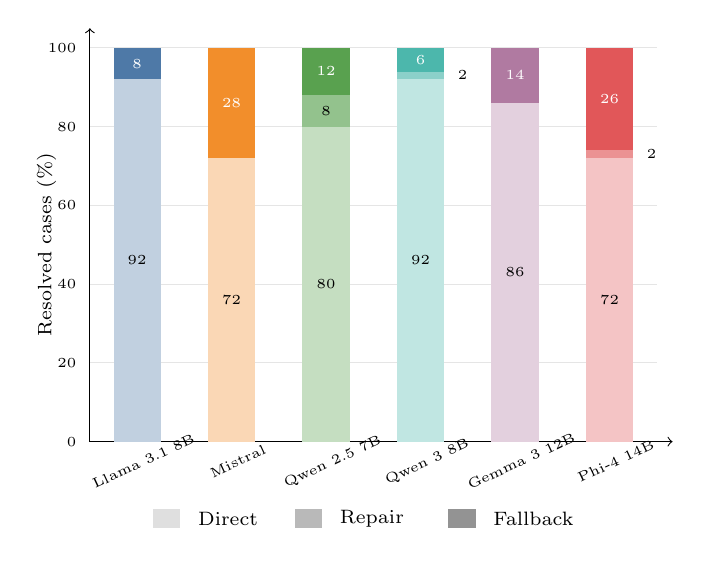
\begin{tikzpicture}
\foreach \y/\lab in {0/0,1/20,2/40,3/60,4/80,5/100}{
    \draw[gray!20] (0.4,\y) -- (7.6,\y);
    \node[anchor=east,font=\tiny] at (0.35,\y) {\lab};
}
\draw[->] (0.4,0) -- (7.8,0);
\draw[->] (0.4,0) -- (0.4,5.25);
\node[font=\scriptsize,rotate=90]
    at (-0.15,2.5) {Resolved cases (\%)};

\fill[LlamaColor!35] (0.70,0.00) rectangle (1.30,4.60);
\fill[LlamaColor] (0.70,4.60) rectangle (1.30,5.00);
\node[font=\tiny] at (1.00,2.30) {92};
\node[font=\tiny,text=white] at (1.00,4.80) {8};
\node[anchor=north,font=\tiny,align=center,rotate=25]
    at (1.00,-0.08) {Llama 3.1 8B};

\fill[MistralColor!35] (1.90,0.00) rectangle (2.50,3.60);
\fill[MistralColor] (1.90,3.60) rectangle (2.50,5.00);
\node[font=\tiny] at (2.20,1.80) {72};
\node[font=\tiny,text=white] at (2.20,4.30) {28};
\node[anchor=north,font=\tiny,align=center,rotate=25]
    at (2.20,-0.08) {Mistral};

\fill[Qwen25Color!35] (3.10,0.00) rectangle (3.70,4.00);
\fill[Qwen25Color!65] (3.10,4.00) rectangle (3.70,4.40);
\fill[Qwen25Color] (3.10,4.40) rectangle (3.70,5.00);
\node[font=\tiny] at (3.40,2.00) {80};
\node[font=\tiny] at (3.40,4.20) {8};
\node[font=\tiny,text=white] at (3.40,4.70) {12};
\node[anchor=north,font=\tiny,align=center,rotate=25]
    at (3.40,-0.08) {Qwen 2.5 7B};

\fill[Qwen3Color!35] (4.30,0.00) rectangle (4.90,4.60);
\fill[Qwen3Color!65] (4.30,4.60) rectangle (4.90,4.70);
\fill[Qwen3Color] (4.30,4.70) rectangle (4.90,5.00);
\node[font=\tiny] at (4.60,2.30) {92};
\node[font=\tiny,text=white] at (4.60,4.85) {6};
\node[font=\tiny,anchor=west] at (4.95,4.65) {2};
\node[anchor=north,font=\tiny,align=center,rotate=25]
    at (4.60,-0.08) {Qwen 3 8B};

\fill[GemmaColor!35] (5.50,0.00) rectangle (6.10,4.30);
\fill[GemmaColor] (5.50,4.30) rectangle (6.10,5.00);
\node[font=\tiny] at (5.80,2.15) {86};
\node[font=\tiny,text=white] at (5.80,4.65) {14};
\node[anchor=north,font=\tiny,align=center,rotate=25]
    at (5.80,-0.08) {Gemma 3 12B};

\fill[PhiColor!35] (6.70,0.00) rectangle (7.30,3.60);
\fill[PhiColor!65] (6.70,3.60) rectangle (7.30,3.70);
\fill[PhiColor] (6.70,3.70) rectangle (7.30,5.00);
\node[font=\tiny] at (7.00,1.80) {72};
\node[font=\tiny,text=white] at (7.00,4.35) {26};
\node[font=\tiny,anchor=west] at (7.35,3.65) {2};
\node[anchor=north,font=\tiny,align=center,rotate=25]
    at (7.00,-0.08) {Phi-4 14B};

\fill[gray!25] (1.20,-1.10) rectangle (1.55,-0.85);
\node[font=\scriptsize,anchor=west] at (1.65,-0.975) {Direct};
\fill[gray!55] (3.00,-1.10) rectangle (3.35,-0.85);
\node[font=\scriptsize,anchor=west] at (3.45,-0.975) {Repair};
\fill[gray!85] (4.95,-1.10) rectangle (5.30,-0.85);
\node[font=\scriptsize,anchor=west] at (5.40,-0.975) {Fallback};
\end{tikzpicture}
}
\caption{Generation outcomes for the 50 resolved cases per model.
Within each model, lighter shading indicates initial acceptance,
medium shading indicates successful repair, and darker shading
indicates deterministic fallback.}
\label{fig:validation_paths}
\end{figure}

\subsection{Comparison with Alternative Execution Modes}

The matched comparison includes three models, 100 cases, and five
execution modes, producing 1,500 executions.
Figure~\ref{fig:mode_comparison} presents mean composite quality with
95\% bootstrap confidence intervals.

DeepCTI achieved mean quality of 0.907 [0.883, 0.930].
RAG once reached 0.808 [0.783, 0.832], equal-evidence one-shot
reached 0.805 [0.774, 0.835], iterative no-memory reached
0.803 [0.776, 0.829], and initial one-shot reached
0.605 [0.563, 0.644].

\begin{figure}[!t]
\centering
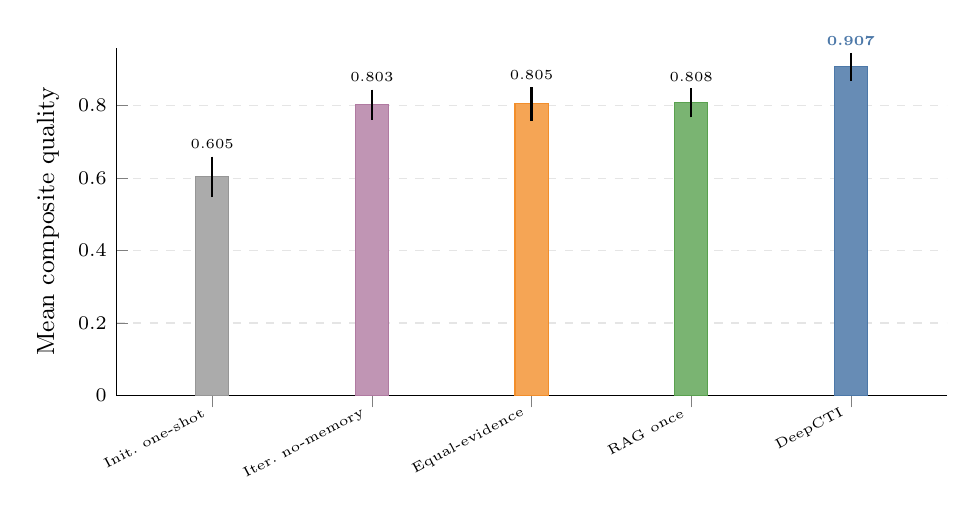
\begin{tikzpicture}
\begin{axis}[
    ybar,
    width=\columnwidth,
    height=6.0cm,
    ymin=0,
    ymax=0.96,
    ylabel={Mean composite quality},
    xtick={1,2,3,4,5},
    xticklabels={
        Init.\ one-shot,
        Iter.\ no-memory,
        Equal-evidence,
        RAG once,
        DeepCTI
    },
    x tick label style={rotate=28,anchor=east,font=\tiny},
    tick label style={font=\scriptsize},
    label style={font=\small},
    ytick={0,0.2,0.4,0.6,0.8},
    ymajorgrids=true,
    xmajorgrids=false,
    grid style={dashed,gray!20},
    axis x line*=bottom,
    axis y line*=left,
    bar width=12pt,
    enlarge x limits=0.15,
    clip=false
]
\addplot+[
    ybar,bar shift=0pt,
    fill=OneShotColor!80,draw=OneShotColor,mark=none,
    error bars/.cd,y dir=both,y explicit,
    error bar style={draw=black,line width=0.8pt},
    error mark options={draw=black,line width=0.8pt}
] coordinates {(1,0.605) += (0,0.039) -= (0,0.042)};

\addplot+[
    ybar,bar shift=0pt,
    fill=NoMemoryColor!80,draw=NoMemoryColor,mark=none,
    error bars/.cd,y dir=both,y explicit,
    error bar style={draw=black,line width=0.8pt},
    error mark options={draw=black,line width=0.8pt}
] coordinates {(2,0.803) += (0,0.026) -= (0,0.027)};

\addplot+[
    ybar,bar shift=0pt,
    fill=EqualEvidenceColor!80,draw=EqualEvidenceColor,mark=none,
    error bars/.cd,y dir=both,y explicit,
    error bar style={draw=black,line width=0.8pt},
    error mark options={draw=black,line width=0.8pt}
] coordinates {(3,0.805) += (0,0.030) -= (0,0.031)};

\addplot+[
    ybar,bar shift=0pt,
    fill=RAGColor!80,draw=RAGColor,mark=none,
    error bars/.cd,y dir=both,y explicit,
    error bar style={draw=black,line width=0.8pt},
    error mark options={draw=black,line width=0.8pt}
] coordinates {(4,0.808) += (0,0.024) -= (0,0.025)};

\addplot+[
    ybar,bar shift=0pt,
    fill=DeepCTIColor!85,draw=DeepCTIColor,mark=none,
    error bars/.cd,y dir=both,y explicit,
    error bar style={draw=black,line width=0.9pt},
    error mark options={draw=black,line width=0.9pt}
] coordinates {(5,0.907) += (0,0.023) -= (0,0.024)};

\node[font=\tiny,anchor=south] at (axis cs:1,0.655) {0.605};
\node[font=\tiny,anchor=south] at (axis cs:2,0.840) {0.803};
\node[font=\tiny,anchor=south] at (axis cs:3,0.845) {0.805};
\node[font=\tiny,anchor=south] at (axis cs:4,0.840) {0.808};
\node[font=\tiny,anchor=south,text=DeepCTIColor]
    at (axis cs:5,0.938) {\textbf{0.907}};
\end{axis}
\end{tikzpicture}
\caption{Mean composite quality in the matched execution-mode
comparison. Error bars show 95\% bootstrap confidence intervals
with the cases as the resampling unit.}
\label{fig:mode_comparison}
\end{figure}

Table~\ref{tab:mode_results} reports applicability accuracy,
completion rate, and median model latency. DeepCTI achieved
applicability accuracy of 1.000, compared with 0.693 for RAG once,
0.680 for equal-evidence one-shot, 0.647 for iterative no-memory,
and 0.290 for initial one-shot. The forbidden-action lexical rate
was 0.00 for every mode and is therefore omitted from the table.

\begin{table}[!t]
\caption{Decision and execution measures in the matched
100-case mode comparison.}
\label{tab:mode_results}
\centering
\scriptsize
\setlength{\tabcolsep}{2.8pt}
\renewcommand{\arraystretch}{1.10}
\begin{tabularx}{\columnwidth}{
    >{\hsize=1.3\hsize\raggedright\arraybackslash}X
    >{\hsize=0.9\hsize\centering\arraybackslash}X
    >{\hsize=0.9\hsize\centering\arraybackslash}X
    >{\hsize=0.9\hsize\centering\arraybackslash}X
}
\toprule
\textbf{Mode} &
\textbf{Applic.} &
\textbf{Complete} &
\textbf{Median Lat. (s)} \\
\midrule
\rowcolor{DeepCTIColor!14}
DeepCTI &
\textbf{1.000} &
\textbf{1.000} &
\textbf{1.56} \\
\rowcolor{RAGColor!14}
RAG once &
0.693 &
0.987 &
7.86 \\
\rowcolor{EqualEvidenceColor!14}
Equal-evidence one-shot &
0.680 &
0.990 &
6.93 \\
\rowcolor{NoMemoryColor!14}
Iterative no-memory &
0.647 &
0.977 &
19.67 \\
\rowcolor{OneShotColor!18}
Initial one-shot &
0.290 &
0.993 &
5.78 \\
\bottomrule
\end{tabularx}
\end{table}

The paired comparisons in Table~\ref{tab:mode_contrasts} show mean
quality improvements of 0.102 over equal-evidence one-shot,
0.099 over RAG once, 0.104 over iterative no-memory, and
0.302 over initial one-shot. All four differences remained
significant after Holm correction.

The equal-evidence condition receives the complete case evidence
in one prompt, so its comparison with DeepCTI controls for total
information availability. The iterative no-memory condition provides
a comparison with repeated generation without retained state.
The results support the complete DeepCTI execution path under these
conditions, including its controller, memory, validation, and fallback.

\begin{table}[!t]
\caption{Paired quality differences between DeepCTI and alternative
execution modes. Positive values favor DeepCTI.}
\label{tab:mode_contrasts}
\centering
\scriptsize
\setlength{\tabcolsep}{2.2pt}
\renewcommand{\arraystretch}{1.10}
\begin{tabularx}{\columnwidth}{
    >{\hsize=1.4\hsize\raggedright\arraybackslash}X
    >{\hsize=0.7\hsize\centering\arraybackslash}X
    >{\hsize=1.0\hsize\centering\arraybackslash}X
    >{\hsize=0.9\hsize\centering\arraybackslash}X
}
\toprule
\textbf{Comparator} &
\textbf{$\Delta Q$} &
\textbf{95\% CI} &
\textbf{$p_{\mathrm{Holm}}$} \\
\midrule
\rowcolor{EqualEvidenceColor!14}
Equal-evidence one-shot &
+0.102 &
[+0.070, +0.137] &
$4.0\times10^{-5}$ \\
\rowcolor{RAGColor!14}
RAG once &
+0.099 &
[+0.073, +0.127] &
$4.0\times10^{-5}$ \\
\rowcolor{NoMemoryColor!14}
Iterative no-memory &
+0.104 &
[+0.077, +0.133] &
$4.0\times10^{-5}$ \\
\rowcolor{OneShotColor!18}
Initial one-shot &
\textbf{+0.302} &
\textbf{[+0.251, +0.355]} &
$4.0\times10^{-5}$ \\
\bottomrule
\end{tabularx}
\end{table}

Action-keyword recall was 0.785 for DeepCTI, compared with 0.605
for RAG once, 0.633 for equal-evidence one-shot, 0.620 for iterative
no-memory, and 0.322 for initial one-shot.

For cases with non-empty information-need references, DeepCTI
achieved information-need keyword recall of 1.000. RAG once,
equal-evidence one-shot, iterative no-memory, and initial one-shot
achieved 0.561, 0.533, 0.569, and 0.361, respectively. These
results show coverage of the expected information-need terms under
the controlled profiles.

\subsection{Efficiency}

Median recorded model latency ranged from 1.62~s for Llama 3.1 8B
to 4.71~s for Phi-4 14B in the six-model experiment. Median token
usage ranged from 509.5 for Llama 3.1 8B to 704.0 for Mistral.
These differences reflect the synthesis and repair calls made by
each model.

In the matched comparison, DeepCTI recorded the lowest median model
latency at 1.56~s. Initial one-shot recorded 5.78~s,
equal-evidence one-shot 6.93~s, RAG once 7.86~s, and iterative
no-memory 19.67~s.

The DeepCTI cost distribution includes the unresolved half of the
dataset, which returns deterministic verification requests without
model calls. These cases record zero model duration and tokens.
The reported medians therefore describe inference usage across
the complete balanced case set, including this controller behavior.

\subsection{Metric Limitation}
\label{sec:metric-limitation}

The contradiction component of composite quality is affected by a
lexical scoring artifact. In uncertain cases, the word
``conflicting'' in the deterministic response can match the
scorer's contradiction cue even when the reference describes missing
information. This reduces the distinction between unresolved
information and contradictory evidence in that component.

The artifact affects composite quality but does not change the
recorded applicability, forbidden-action lexical rate, or completion
results. Individual measures are therefore considered alongside
the aggregate score when interpreting the controlled comparison.

\section{Discussion and Limitations}

The controlled study supports explicit evidence-state management for
CTI-driven mitigation decision support. Applicability remained consistent
across six language models, while response quality and inference cost
varied with the synthesis model. The matched comparison also showed
higher composite quality for DeepCTI than the evaluated alternatives,
including equal-evidence one-shot and iterative no-memory. Together,
these findings support the combined use of structured memory,
deterministic decision rules, and response validation under staged
observations. For RQ-1, the study illustrates how this design connects
local facts to applicability assessments and verification needs.

Operational use requires the evidence supporting an assessment to
remain current. Asset identity, collection time, and provenance should
help identify when configuration changes require
reassessment~\cite{johnson2011configuration,dempsey2011monitoring}.
For RQ-2, a supported judgment should inform a separate authorization
check before tool execution. A version query may be permitted while
a restart requires approval and a maintenance window. Attribute-based
access control and agent runtime controls provide foundations for
evaluating these conditions~\cite{hu2014abac,shi2025progent,wang2026agentspec}.

The next evaluation should use independently reviewed cases with
changing configurations, conflicting observations, and contextual
permissions. Matched baselines should receive the same initial evidence,
available tools, permissions, and acquisition budget. Measures should
cover evidence-need identification, recommendation support, decision
progress, authorization compliance, and completion of permitted actions.
The benchmarks reviewed in Section~II can complement these cases
through evaluation of individual CTI and agent capabilities.

The present study uses synthetic local profiles, generated references,
and predefined evidence stages. Its findings concern these controlled
conditions. Lexical checks provide bounded response measures, and the
contradiction-scoring artifact described in
Section~\ref{sec:metric-limitation} affects composite quality. Recorded
latency represents model-call duration rather than total investigation
time. Live evidence verification and enforcement of execution permissions
remain the operational extensions identified by this agenda.

\section{Conclusion}

We argue that CTI-driven mitigation should be governed by an explicit
evidence state connecting local applicability, unresolved information,
and newly obtained observations. Investigative and mitigation actions
should additionally depend on organizational policy and current
operational context.

DeepCTI implements evidence-state management through source-linked
observations, structured fact memory, deterministic decision control,
and validated language-model synthesis. The controlled study across
six local models and the matched execution-mode comparison provide
preliminary evidence that this combined design improves response
quality under staged observations.

The framework and findings provide a basis for extending mitigation
decision support to changing environments. Future work will examine
current-state verification, evidence reconciliation, and contextual
authorization through independently reviewed operational cases.


\bibliographystyle{unsrt}
\bibliography{deepcti_references}

\end{document}